\documentclass[oneside,final,14pt,a4paper]{extreport}


%=====================================================================
%  BACHELOR THESIS PROPOSAL (REVISED after supervisor feedback)
%=====================================================================


\usepackage[T1]{fontenc}
\usepackage[utf8]{inputenc}
\usepackage[english]{babel}
\usepackage{tempora}

% Monospaced font: Courier (bold available via psnfss).
% The former manual \DeclareFontShape{OT1}{cmtt}{bx}{n}{...} was dead code:
% with \ttdefault=pcr it was never used, so it has been removed.
\renewcommand{\ttdefault}{pcr}

% Micro-typographic adjustments: reduce overfull lines caused by long
% identifiers and 14 pt setting, without changing the font size.
\usepackage{microtype}
\setlength{\emergencystretch}{2em}


\usepackage{vmargin}
\setpapersize{A4}
\setmarginsrb{2.5cm}{2.2cm}{2.2cm}{2.2cm}{0pt}{10mm}{0pt}{13mm}
\usepackage{setspace}
\setstretch{1.0}
\usepackage{indentfirst}
\parindent=1.25cm


\usepackage{amsmath,amsfonts}
\usepackage{amsthm}
\usepackage{upgreek}
\usepackage{bm}


\usepackage{xcolor}
\usepackage{graphicx}
\graphicspath{{figs/}}
\usepackage{float}
\usepackage{array}
\usepackage{multirow}
\usepackage{booktabs}
\usepackage{longtable}
\usepackage[font=singlespacing,labelfont=bf]{caption}
\usepackage{subcaption}
\usepackage{enumitem}


\usepackage{tikz}
\usetikzlibrary{positioning,arrows.meta}


\usepackage{csquotes}
\usepackage[backend=biber,style=ieee,autocite=inline]{biblatex}
\addbibresource{references.bib}
\DefineBibliographyStrings{english}{%
  bibliography = {References},}


\usepackage{chngcntr}
\usepackage{pdfpages}
\usepackage{placeins}
\usepackage{fancyhdr}


\captionsetup[table]{labelfont={normalfont}, name={TABLE}, labelsep={newline}}
\captionsetup[figure]{labelfont={normalfont}, name={Fig.}, labelsep=period}


\renewcommand{\thesection}{\arabic{section}}
\counterwithin{figure}{section}
\counterwithin{table}{section}
\counterwithin{equation}{section}
\setcounter{secnumdepth}{3}


\setlength{\headheight}{32.0976pt}

% Modern fancyhdr interface (replaces the deprecated fancyplain style,
% preserving the original header layout for this oneside document:
% left header = section mark, right header = page number, empty footer).
% \pagestyle{fancy}
% \fancyhf{}
% \renewcommand{\sectionmark}[1]{\markright{\thesection\ #1}}
% \fancyhead[L]{\bfseries\rightmark}
% \fancyhead[R]{\bfseries\thepage}
% \renewcommand{\headrulewidth}{0.4pt}


\usepackage{hyperref}
\hypersetup{colorlinks=true, linkcolor=black, citecolor=black, urlcolor=black}


\begin{document}

\begingroup
\setlength{\parindent}{0pt}
\setlength{\parskip}{0pt}

\begin{center}
    {\Large\bfseries
    Confidence-Aware Adaptive Verification of LLM Recommendations\\
    in Introductory Programming Tasks\par}
    \vspace{0.5em}
    {\normalsize Student: Lidia Davydova\par}
    \vspace{0.15em}
    {\normalsize Supervisor: Paolo Ciancarini\par}
\end{center}

\vspace{0.5em}

\begingroup
\small
\begin{minipage}{0.9\textwidth}
\noindent\textbf{Abstract.}
Large language models (LLMs) are increasingly used in programming
education, but their recommendations can be plausible yet incorrect,
so the quality of human--AI collaboration depends on
\emph{appropriate reliance}: accepting correct recommendations and
rejecting incorrect ones. Verification support can help users evaluate
recommendations, and introductory programming is well suited to it
because correctness can be checked through independent, execution-based
evidence such as tests, traces, and counterexamples. Providing such
evidence on every trial, however, introduces unnecessary interaction
cost. This thesis investigates whether a simple, interpretable adaptive
policy---gating verification availability on the participant's
\emph{prior-answer confidence}---can reduce verification effort relative to
always-available verification. The gate is motivated by a simple mechanism:
participants who are unsure of their own answer are more likely to defer to
the recommendation \cite{YanivKleinberger2000}, so independent evidence is
most valuable exactly there.
The human--AI interaction is specified through an explicit \emph{escalation
rule} that fixes who recommends, who supplies independent verification
evidence, who decides, and what is recorded; the three experimental
conditions are three escalation policies within that single specification. A
within-subject experiment (provisional $N=60$) compares no-verification,
static, and adaptive conditions on a benchmark of 18 introductory Python
tasks with frozen, pre-validated Qwen3-8B recommendations balanced between
correct and incorrect. The two primary outcomes are final-answer accuracy and
verification effort; reliance measures are secondary. Reliance on the LLM is
distinguished from agreement with an answer the participant already held.
The accuracy claim has two parts: adaptive verification is tested for
non-inferiority against static verification and for superiority against no
verification, including the boundary case of confident but mistaken
participants. Expected contributions include trial-level evidence on the
effort--quality trade-off of confidence-gated verification, a validated
reproducible benchmark with an instrumented prototype, and a complete
analysis pipeline.
\end{minipage}
\endgroup

\vspace{0.5em}
\endgroup

%=====================================================================
\section{Introduction and Research Problem}
%=====================================================================


Large language models (LLMs) are increasingly used in programming education
and software engineering to generate, explain, and debug code and to propose
answers to tasks \cite{Ma2024,Cambaz2024,Denny2024}. Because such systems can
produce plausible but incorrect outputs, the quality of the joint human--AI
outcome depends not only on model accuracy but on \emph{appropriate reliance}
\cite{LeeSee2004}: accepting correct recommendations and rejecting incorrect
ones. Over-reliance and under-reliance are the corresponding failures
\cite{PoursabziSangdeh2021,Vasconcelos2022}.


Verification support can help users evaluate recommendations, and programming
tasks suit it well: correctness can often be checked independently through
execution, tests, traces, or counterexamples---evidence grounded in the task
itself rather than in another LLM-generated justification. This matters
because explanations assist only when users can interpret them and connect
them to the recommendation, and simply providing more information does not
automatically reduce over-reliance
\cite{Bucinca2021,Vasconcelos2022,Bo2025,Schemmer2022}. Moreover, one can
only verify an answer one has the grounding to check \cite{Zhang2024Verify};
introductory programming provides exactly such grounding. However,
verification on every trial introduces unnecessary interaction cost, which
motivates providing verification evidence \emph{selectively}
\cite{CascadedLM2025}.


\subsection{Research Problem}

The research problem is how to provide verification support selectively, using
only information available before the correctness of the LLM recommendation is
known. The thesis investigates whether a simple adaptive policy, based
primarily on the user's \emph{prior-answer confidence}, can provide independent
verification support at lower effort than always-available verification, and
how verification effort trades off against decision quality. The focus is a
simple, interpretable policy---not a new LLM, a new verification algorithm, or
an optimisation method. The contribution is therefore not the threshold rule
itself; it is the controlled empirical evaluation of whether a simple
confidence gate can reduce verification exposure while preserving final-answer
accuracy and appropriate reliance compared with always-available and
no-verification baselines.

\subsection{Analytical Framing}
\label{subsec:framing}

The human--AI interaction is specified through an explicit \emph{escalation
rule} \cite{Ciancarini2027}: who recommends, who supplies independent
verification evidence, who decides, and what is recorded. The three
experimental conditions are three escalation policies within that single
specification, so the recommender, the evidence provider, the decider, and the
audit record are held fixed and only the routing of evidence changes.
Section~\ref{subsec:design} states the rule and its instantiation in the
study; Section~\ref{subsec:policy} states the confidence gate.

The rule is used as a specification device, not as a claim that the study
instantiates a full coordination model. There is a single decision-maker, a
frozen recommender that neither negotiates nor reallocates work, and no
multi-agent task allocation. The empirical question is when independently
produced evidence reaches the person who decides.


%=====================================================================
\section{Research Questions}
%=====================================================================


\textbf{RQ1 (accuracy, primary).} What is the effect of confidence-gated
adaptive verification on final-answer accuracy relative to (a)~always-available
static verification and (b)~no verification?

\textbf{RQ2 (effort, primary).} What is the effect of confidence-gated
adaptive verification on participant-level verification
effort---evidence-examination rate,
evidence-examination time, and total decision time---relative to
always-available static verification?

\textbf{RQ3 (exploratory).} How do the accuracy and effort effects of the
adaptive policy vary with prior-answer confidence, task type, and
the confident-but-mistaken stratum (Section~\ref{subsec:blindspot})?

These questions correspond to three pre-specified tests. The adaptive-versus-static
accuracy contrast is a one-sided non-inferiority test against the margin
$\delta_Q$ (Section~\ref{subsec:quality}); the adaptive-versus-no-verification
accuracy contrast is a superiority test; and the effort contrast between
adaptive and static is a one-sided superiority test in the direction of reduced
effort, the primary test of RQ2. The static-versus-no-verification
contrast is reported as a benchmark for interpreting the other two. Reliance
measures (Section~\ref{subsec:metrics}) are secondary outcomes, distinguishing
true reliance on the LLM from agreement with an answer the participant already
held.

Neither task type nor task difficulty is an input to the adaptive policy
(Section~\ref{subsec:policy}); both are analysed only as exploratory
moderators of policy effectiveness.

A policy premise check examines whether prior-answer confidence is associated
with initial-answer correctness (Section~\ref{subsec:premise}), and a
non-inferiority test establishes whether adaptive verification preserves
decision quality relative to static verification
(Section~\ref{subsec:quality}).


%=====================================================================
\section{Novelty and Contributions}
%=====================================================================


The novelty is \emph{not} the observation that confidence relates to reliance
on AI---miscalibration is well documented \cite{KrugerDunning1999,Bo2025} and
taken here as a premise---but the combination of elements usually studied in
isolation: (i)~confidence as a per-trial \emph{trigger} deciding \emph{when}
support is shown, rather than an outcome to be calibrated or an AI-side
uncertainty signal; (ii)~\emph{independent, execution-based} evidence (tests,
traces, counterexamples) rather than additional AI-generated explanations;
(iii)~a programming setting in which recommendations are pre-validated and
objective evidence exists; and (iv)~an explicit effort--quality trade-off
evaluation, treating verification effort as a first-class outcome
\cite{CascadedLM2025,Zhang2024Verify}.


The thesis is expected to contribute: (1)~trial-level empirical evidence,
analysed with mixed-effects models, on whether a simple confidence-based
policy reduces verification effort while preserving final-answer accuracy
(RQ1--RQ2); (2)~an explicit escalation rule that states who recommends, who
provides evidence, who decides, and what is recorded, and that treats the three
conditions as three escalation policies within one specification
\cite{Ciancarini2027}; (3)~a validated benchmark of 18 introductory Python
tasks with fixed, pre-validated LLM recommendations (balanced
correct/incorrect), task-type and difficulty labels, and verification data;
(4)~a reproducible prototype of the three conditions with complete logging,
including evidence examination; (5)~an analysis pipeline for the primary
outcome and effort measures.
The contribution is deliberately not a new LLM, a new algorithm, or a
tutoring system: the confidence gate is intentionally simple, and its value
lies in the controlled empirical comparison against always-available and
no-verification baselines in a reproducible human--AI interaction experiment.

%=====================================================================
\section{State-of-the-Art}
%=====================================================================

\paragraph{Trust and appropriate reliance.}
Trust in automation is classically defined as the attitude that an agent will
help an individual achieve a goal under uncertainty and in risky situations,
and the design goal is \emph{appropriate} reliance rather than maximal trust
\cite{LeeSee2004}. In AI-assisted decision-making, users frequently fail to
calibrate reliance to recommendation quality: over-reliance on incorrect
advice and under-reliance on correct advice persist even when additional
information about the model is available
\cite{PoursabziSangdeh2021,Chen2023}. Comparable miscalibration between
confidence and correctness is documented for human judgment itself
\cite{KrugerDunning1999}.

\paragraph{Explanations and cognitive forcing.}
Cognitive forcing functions, which compel deliberate engagement with AI
advice before it is accepted, can reduce over-reliance \cite{Bucinca2021}.
However, meta-analytic evidence finds no reliable benefit of explanations
over AI predictions alone \cite{Schemmer2022}, and experimental work shows
that explanations reduce over-reliance only when they are interpretable and
help users anticipate AI errors \cite{Vasconcelos2022}; interventions
evaluated with LLM advice similarly reduced over-reliance without improving
appropriate reliance overall \cite{Bo2025}. Because explanation-based
support may itself provide additional AI-generated information, this
motivates verification support grounded in independent, execution-based
evidence rather than additional AI text.

\paragraph{Verification and its cost.}
Correctness alone is an insufficient evaluation criterion: human scrutiny of
AI outputs is valuable but consumes time and effort, which motivates
frameworks that invoke human input selectively \cite{CascadedLM2025}.
Introductory programming supplies the grounding that verification requires:
executable reference answers, tests, and traces make objective evidence
available at decision time \cite{Zhang2024Verify}.

\paragraph{Confidence as a signal for adaptive support.}
Closest to this thesis, \cite{Bo2025} evaluate interventions for reliance on
LLM advice and find that interventions reduce over-reliance but generally
fail to improve appropriate reliance, while users' confidence is poorly
calibrated. The authors discuss confidence calibration as a design
implication. Related work adapts support to the user's trust state
\cite{SrinivasanAdjustForTrust}. Here, prior-answer confidence is instead an
\emph{input signal}: a lightweight trigger deciding \emph{when} independent
support is shown, leaving the user's internal state unchanged. The documented
relationship between confidence and correctness is taken as a premise: if
confidence carries information about correctness, it can also inform when
verification is worth its interaction cost---an effort dimension absent from
calibration-oriented work and a primary outcome here (RQ2).

\begin{table}[t]
\centering
\caption{Positioning relative to the closest lines of work.}
\label{tab:positioning}
\footnotesize
\begin{tabular}{@{}>{\raggedright\arraybackslash}p{2.7cm}>{\raggedright\arraybackslash}p{2.3cm}>{\raggedright\arraybackslash}p{2.9cm}>{\raggedright\arraybackslash}p{3.5cm}>{\raggedright\arraybackslash}p{2.7cm}@{}}
\toprule
Work & Signal & What is gated & Evidence & Primary outcome \\
\midrule
Bo2025 & None (intervention type) & Reliance intervention &
Accuracy or explanation & Appropriate reliance \\
Srinivasan et al. & User trust state & Explanation type; forced pause &
AI explanations & Inappropriate reliance \\
Zhang2024Verify & Decision difficulty & Feature explanation &
Feature attributions & Over-reliance \\
CascadedLM2025 & Model confidence and cost & Human review &
Model cascade & Cost and accuracy \\
This thesis & Prior-answer confidence & Independent execution evidence &
Tests, traces, counterexamples & Accuracy and effort \\
\bottomrule
\end{tabular}
\end{table}

Table~\ref{tab:positioning} makes the combination claimed as novel explicit:
each element exists separately, but no prior study gates \emph{independent,
execution-based} evidence on the decider's own prior confidence and treats
interaction effort as a primary outcome.

\paragraph{Coordination and governance of LLM-based systems.}
Because a language model can produce a fluent answer without guaranteeing that
it is correct, in scope, or compatible with other decisions, plausible but
unsupported output must be managed by the surrounding system rather than
trusted on fluency alone \cite{Ciancarini2027}. Recent work on agentic software
engineering argues that autonomy increases, rather than reduces, the need for
coordination: claims may need to be checked against artefacts, actions against
permissions, and decisions against explicitly assigned authority, and shared
artefacts, logs, tests, and approval points make decisions traceable
\cite{Ciancarini2027}. Coordination determines, among other things, the
escalation paths of a system: who supplies evidence, who decides, and under
whose authority. This motivates the explicit escalation rule adopted here
(Section~\ref{subsec:design}), in which independent execution-based evidence
replaces reliance on conversational
output alone.

\paragraph{LLM assistance in programming and research gap.}
LLMs are increasingly used for code generation, debugging, and explanation in
computing education \cite{Ma2024,Cambaz2024,Denny2024}, but can be plausible
yet incorrect, so users must evaluate recommendations critically. Prior work
establishes that intuition, explanation design, and decision difficulty shape
reliance \cite{Chen2023,Vasconcelos2022,Zhang2024Verify}; what remains
unknown is whether a participant's prior-answer confidence can serve as a
lightweight trigger for selectively displaying \emph{independent verification
evidence} after an LLM recommendation in introductory programming
tasks---the gap addressed here.


%=====================================================================
\section{Goal of the Thesis}
%=====================================================================

The goal of the thesis is to design, implement, and empirically evaluate an
experimental system that provides selective verification support for LLM
recommendations in introductory programming tasks. The study has two primary
outcomes---final-answer accuracy and verification effort---and investigates
whether a simple confidence-based adaptive policy can reduce verification
effort while preserving decision quality relative to an always-available
(static) policy.

The project schedule is provided in Section~\ref{sec:workplan}.

\subsection{The Escalation Rule}
\label{subsec:design}

Coordination, in the account of Ciancarini \cite{Ciancarini2027}, determines
among other things the escalation paths of a system: who supplies evidence, who
decides, and under whose authority, so that correct and incorrect
recommendations are managed by the surrounding system rather than by
conversation alone. The study adopts that element as an explicit
\emph{escalation rule}. The rule does not add a new component; it makes
explicit the routing already implied by the design. Table~\ref{tab:escalation}
maps its parts onto the study.

The three experimental conditions are therefore \emph{three escalation policies
within the same specification}: only the escalation rule changes, while the
recommender, the evidence provider, the decider, and the audit record are held
fixed. This keeps the system components unchanged and makes the comparison a
comparison of escalation policies rather than of different systems. Decision
authority is never reassigned: the participant decides in every condition, and
only the flow of evidence is conditional.

The rule is a specification device, not a claim that the study instantiates a
full coordination model: there is one decision-maker, a frozen recommender that
neither negotiates nor reallocates work, and no multi-agent task allocation.
The empirical question is when independently produced evidence reaches the
person who decides.

\begin{table}[H]
\centering
\caption{The escalation rule and its instantiation in the study.}
\label{tab:escalation}
\small
\begin{tabular}{@{}>{\raggedright\arraybackslash}p{2.6cm}>{\raggedright\arraybackslash}p{7.4cm}>{\raggedright\arraybackslash}p{4.2cm}@{}}
\toprule
Role & Instantiation & Recorded artefact \\
\midrule
Recommender & Fixed, offline Qwen3-8B snapshot; no access to condition,
policy, or participant & Model hash, prompt, raw output \\
Evidence provider & Researchers; execution-based tests, traces, and
counterexamples derived from the task and reference answer, never from the
recommender & Verification artefacts and their expected outcomes \\
Decider & Participant records an initial answer, a prior-answer confidence
rating, and a final judgment & Responses, confidence, timestamps \\
Escalation rule & Static: evidence always; adaptive: evidence iff $c<\tau$;
no verification: never & Availability flag, policy decision, timestamp \\
Audit and record & Instrumented prototype logs the trial; the correctness
label is analysis-only and never shown & Trial-level log and analysis
dataset \\
\bottomrule
\end{tabular}
\end{table}


\subsection{Task Domain and Benchmark}
\label{subsec:answerspace}

The benchmark comprises 18 introductory Python programming tasks 
of three types: \emph{identify bug}, \emph{check against specification}, 
and \emph{select correct implementation}. ``Write or repair code'' 
tasks are excluded because they do not provide a sufficiently constrained 
response space for the primary reliance measures.

The benchmark metadata include task type, difficulty level, reference answer,
fixed LLM recommendation, recommendation correctness, and task-specific
verification data. The 18 LLM recommendations are balanced between nine
correct and nine incorrect recommendations. Correct and incorrect
recommendations are distributed across the three task types as evenly as the
benchmark construction permits.

\emph{Task difficulty.} Each task is assigned a difficulty level
(\emph{low}, \emph{medium}, or \emph{high}) before the main experiment
according to a predefined rubric based on code complexity, the number of
reasoning steps required, and the programming constructs involved. Difficulty
ratings are checked during the pilot against pilot accuracy and response
times and are frozen together with the benchmark. Difficulty is not used as
an input to the adaptive policy and is analysed only as an exploratory
factor; if the pilot indicates that the ratings are unreliable, difficulty is
dropped from the confirmatory analysis and retained only as descriptive
metadata.

Each task has a closed-form response space that makes correctness 
and changes in the participant's answer well-defined. For \emph{identify bug}, 
the response consists of a binary bug-presence judgment and, when a bug 
is present, a line number identifying its location. Optional free-text 
explanations are recorded only for qualitative analysis. 
For \emph{check against specification}, the response is a binary 
\texttt{COMPLIANT}/\texttt{NOT\_COMPLIANT} judgment. 
For \emph{select correct implementation}, the response is an identifier 
corresponding to one of a fixed set of candidate implementations.

\emph{Canonical responses and equality.} Each task defines a canonical response
tuple and an accepted-equivalence set. For \emph{identify bug} the tuple is
(bug presence, line identifier), and a task may accept more than one line when
the bug spans a region; a judgment without a line is scored separately from a
judgment with a line. For \emph{check against specification} the tuple is the
binary judgment. For \emph{select correct implementation} the tuple is the
candidate identifier. Correctness and the equality relations used in
Section~\ref{subsec:metrics} are evaluated on the canonical tuple, never on
free text. The LLM recommendation is rendered through the same response widget
and with the same option labels as the participant's response, so that the
initial answer, the recommendation, and the final answer are directly
comparable and no letter remapping can occur.

\emph{Design and counterbalancing.} Each participant completes all 18 tasks,
with six trials assigned to each experimental condition. Each condition
contains two tasks of each of the three task types, and within each condition
three trials contain correct and three contain incorrect LLM recommendations,
with one of each per task type. Condition-to-task assignment uses a balanced
design with three rotation groups: across the three groups, each task appears
exactly once in each condition. Condition order is counterbalanced with six
sequences combining the three rotations and two orderings; task order within a
condition block is randomized per participant. Two practice trials precede the
experiment and are not analysed.

Because condition membership varies within task across participants and the
rotations are balanced, task-level heterogeneity is not systematically
confounded with the experimental condition, allowing task to be included as a
random effect in the analysis models.

\subsection{LLM Recommendation Specification}
\label{subsec:llm-spec}

All LLM recommendations are generated offline before the main experiment. No
LLM generation is performed during participant trials. Consequently, all
participants receive the same frozen recommendation for a given task, and
differences between experimental conditions cannot be attributed to runtime
LLM sampling variance.

\emph{Model and version.}

The recommendation generator is a fixed local snapshot of a specific
\texttt{Qwen3-8B} model artifact, an 8.2B-parameter instruction-tuned model
distributed by Qwen. The experiment uses an 8-bit quantized model in GGUF
format (\texttt{Q8\_0}). The exact model file, model revision, quantization,
inference backend, software version, and model-file SHA-256 hash are recorded
and frozen before benchmark generation. The benchmark therefore refers to a
specific frozen model artifact rather than to the mutable upstream
\texttt{Qwen3-8B} model name.

\emph{Inference configuration.}

Qwen3 is used in non-thinking mode so that generated recommendations contain
only the requested answer and do not depend on a model-generated reasoning
trace. The generation configuration is fixed as follows:

\begin{verbatim}
model: Qwen3-8B model artifact, 8-bit Q8_0
thinking: disabled
temperature: 0.7
top_p: 0.8
top_k: 20
max_tokens: 256
frequency_penalty: 0
\end{verbatim}

The sampling parameters \texttt{top\_k} and \texttt{frequency\_penalty} are
backend-dependent; their concrete semantics are those of the archived backend
version.

\emph{Reproducibility.}

The exact inference backend and version, command-line options, context
length, and hardware configuration are archived with the benchmark. The
generation seed is archived when supported by the inference backend. Because
GPU inference may be nondeterministic even under a fixed seed, reproducibility
of the benchmark is defined with respect to the archived model artifact and
the archived generation outputs rather than bit-exact regeneration.

\emph{Hardware configuration}
\begin{verbatim}
VRAM: Tesla V100 16 GB
RAM: 128 GB
\end{verbatim}

\emph{Prompt template.}

For each task, the model receives a structured prompt containing:
(i) the task type and instructions, (ii) the task description and any Python
code snippet, (iii) a strict output schema, and (iv) an instruction to return
only the requested answer.

The prompt does not contain information about the experimental condition,
verification policy, participant confidence, or intended correctness of the
recommendation. The complete prompt template and all task-specific prompts are
archived with the benchmark.

\emph{Candidate generation.}

For each benchmark task, multiple candidate LLM recommendations are 
generated using a fixed inference configuration. The model receives 
a task-specific prompt containing the task description, required instructions, 
and a strict output format corresponding to the task's predefined response 
space. The model is instructed to solve the task and return only the 
requested answer, without explanations or confidence estimates.

The LLM recommendation is a task-specific structured answer expressed 
in the predefined response space of the task. For example, 
for an \emph{identify bug} task, it 
may be a predefined bug location or type (e.g., \texttt{LINE\_3}); 
for a \emph{check against specification} task, it may be a binary judgment 
such as \texttt{SATISFIES} or \texttt{DOES\_NOT\_SATISFY}; and for a 
\emph{select correct implementation} task, it may be an implementation 
identifier such as \texttt{B}. The exact response representation is defined 
separately for each task before candidate generation.

Each model output is parsed into the task's canonical structured response 
representation. Outputs that cannot be parsed unambiguously are rejected 
and regenerated. Candidate recommendations are then evaluated against the 
reference answer to determine their correctness.

For each task, one recommendation is selected for the final benchmark. 
The benchmark contains an equal number of correct and incorrect recommendations. 
Correct recommendations must correspond to the reference answer. Incorrect 
recommendations must be objectively incorrect while remaining sufficiently 
plausible to a novice participant. Selection is performed before the participant 
study and does not depend on participant data or experimental condition.

The final recommendation is fixed for the entire study: the same task always 
uses the same LLM recommendation regardless of experimental condition or 
participant. The recommendation is stored in canonical structured form for 
analysis and rendered in a participant-facing form appropriate to the task type.

For correct-recommendation tasks, one valid candidate is selected. For
incorrect-recommendation tasks, an incorrect candidate is selected only if it
is both objectively incorrect and sufficiently plausible to a novice
participant. If no suitable incorrect candidate is produced by the model, the
benchmark construction protocol permits a documented minimal perturbation of
a correct answer, such as an off-by-one value, a wrong operator, or another
task-appropriate error. Such perturbations are recorded separately from
model-generated candidates. The benchmark documentation reports how many of
the 18 recommendations are model-generated and how many are model-seeded;
model-seeded items are excluded from the primary analysis and the full set is
reported as a sensitivity analysis.

\emph{Validation procedure.}

Recommendation correctness is first established automatically whenever an 
objective reference procedure is available. Depending on the task type, this 
may involve program execution, reference-output comparison, or predefined tests. 
When automatic validation is not applicable, correctness is established by comparison 
with the predefined reference answer.

The resulting correctness label and the plausibility of incorrect 
recommendations are then independently reviewed by two annotators with 
introductory programming expertise. Plausibility is rated on a pre-registered
five-point scale (1 = obviously wrong, 5 = indistinguishable from a correct
answer); an incorrect recommendation is retained only if its mean rating is at
least 3 and neither annotator rates it below 2. Inter-rater agreement is
reported with Cohen's $\kappa$ for the correctness label and for the
plausibility threshold. Annotators do not receive information
about the experimental condition or the adaptive policy. Disagreements are
resolved by a third annotator according to the predefined validation procedure.

An incorrect recommendation is retained only when it is objectively incorrect 
and judged sufficiently plausible that its incorrectness is not immediately 
obvious to a novice participant. The validation procedure, candidate pool, 
selected candidate, correctness label, annotator decisions, and any 
perturbation are archived.

After validation, the benchmark is frozen. No recommendation, correctness 
label, prompt, model parameter, or candidate-selection decision is changed 
during the main experiment. Recommendation correctness is hidden from 
participants and is never provided to the adaptive policy. The correctness
label is stored only in the analysis dataset and is not available to the
participant-facing application or to the policy module during a trial.


\subsection{Verification Support and Effort Instrumentation}
\label{subsec:burden}

For each task, the verification mechanism is fixed before the experiment 
and is identical across experimental conditions. The only manipulated factor 
is whether the verification evidence is made available to the participant.

Verification is task-specific and provides independent evidence that 
can be used to evaluate the LLM recommendation. For \emph{identify bug} tasks, 
the system provides predefined tests with failing cases or concrete 
counterexamples that provide evidence about the presence and location of a bug. 
For \emph{check against specification} tasks, the system provides 
specification-based test cases with expected and actual results. For 
\emph{select correct implementation} tasks, the candidate implementations are 
executed against a predefined test suite, and the resulting test outcomes are 
displayed.

Verification artifacts are constructed during benchmark development 
by the researchers and are derived independently from the reference answer 
and task specification. They are not generated by the LLM used to produce 
the experimental recommendations. Each verification artifact has a predefined 
expected outcome and is validated before the main experiment.

For \emph{identify bug} tasks, the researchers construct a set of targeted 
test cases or counterexamples designed to expose the specified bug and provide 
evidence about its location or effect. For \emph{check against specification} 
tasks, the researchers construct specification-based test cases covering the 
relevant requirements, with expected results derived from the task 
specification. For \emph{select correct implementation} tasks, the 
researchers construct a predefined test suite containing cases that 
distinguish the candidate implementations, with expected outcomes derived 
from the task requirements.

Each verification artifact is evaluated against the reference answer or 
reference implementation during benchmark validation. The verification 
artifacts are then independently reviewed by two annotators with introductory 
programming expertise to confirm that they are correct, relevant to the task, 
and sufficient to provide evidence for the intended judgment. Disagreements 
are resolved by a third annotator according to the predefined validation 
procedure.

After validation, the verification artifacts are frozen together with the 
benchmark. No test case, expected result, counterexample, or other verification 
artifact is modified during the main experiment.

The verification mechanism does not explicitly state whether the LLM recommendation 
is correct and does not provide an alternative LLM judgment. Instead, 
it provides task-specific evidence from which participants can assess 
whether the recommendation is consistent with the observed behaviour 
or the task requirements. The evidence therefore does not display the
correctness label used by the experimenter.

It can nevertheless make the correct answer derivable. For
\emph{select correct implementation}, showing test outcomes for every
candidate identifies the candidate that passes; for some bug tasks, a trace
localises the fault unambiguously. Each verification artefact is therefore
labelled \emph{partial} (it narrows the space but does not settle the answer)
or \emph{decisive} (it uniquely determines the correct answer) by two
annotators, with agreement reported as Cohen's $\kappa$. The benchmark
deliberately includes both kinds, diagnosticity is reported in the benchmark
documentation, and it is analysed as an exploratory moderator. This prevents
the study from silently becoming a test of compliance with decisive evidence.

Verification cost and verification effort are treated as distinct concepts. 
Verification cost refers to the intrinsic effort required to establish the 
correctness of a recommendation. Because this latent quantity cannot be observed 
directly from participant behaviour---for example, a participant may stop 
before establishing correctness or may reach an incorrect conclusion---the 
study does not claim to measure intrinsic verification cost.

Instead, the experiment measures observable verification effort, separated by
level. Table~\ref{tab:measures} defines each measure and its role in the
analysis. The umbrella term is \emph{verification effort}; \emph{availability}
always refers to the system, \emph{examination} to the participant, and the
two time measures are distinct constructs. The term \emph{verification time}
is deliberately avoided because it conflates system-level provision of
evidence with participant-level use of evidence.

\begin{table}[t]
\centering
\caption{Verification effort measures, their level, and their role.}
\label{tab:measures}
\small
\begin{tabular}{@{}>{\raggedright\arraybackslash}p{3.9cm}>{\raggedright\arraybackslash}p{1.9cm}>{\raggedright\arraybackslash}p{5.5cm}>{\raggedright\arraybackslash}p{2.7cm}@{}}
\toprule
Measure & Level & Definition & Role \\
\midrule
Verification availability (VAR) & System &
Share of trials on which evidence is offered & Manipulation check \\
Evidence-examination rate & Participant &
Share of available trials on which the panel is examined &
Primary effort outcome \\
Evidence-examination time & Participant &
Seconds the evidence panel is active and focused & Primary effort outcome \\
Total decision time & Participant &
Seconds from recommendation to final judgment & Primary effort outcome \\
Post-availability decision time & Participant &
Seconds from availability to final judgment (available trials only) &
Secondary, conditional \\
Unexamined-evidence share & Participant &
Available but not examined, over available & Descriptive \\
Answer-change rate & Participant &
Final answer differs from initial answer & Descriptive \\
\bottomrule
\end{tabular}
\end{table}

The experimental application records evidence-panel visibility events, 
activation and dismissal timestamps, scrolling and interaction events, 
and the timestamp of the final judgment. Evidence examination is 
operationalised using a rule specified before the main experiment: a trial 
is classified as \emph{evidence-examined} if the evidence panel remains 
active for at least $\delta$ seconds or if the participant performs a 
predefined interaction with the evidence panel. The value of $\delta$ is 
fixed during the pilot and frozen before the main experiment.

This instrumentation distinguishes system-level verification availability 
from participant-level evidence use. Evidence that is made available but 
not examined is still counted as verification availability, but is classified 
as non-examined at the participant level. Consequently, the adaptive condition 
can be evaluated not only by whether verification was made available less often 
than under static verification, but also by whether participants actually 
used the evidence when it was provided.

\subsection{Adaptive Verification Policy}
\label{subsec:policy}

The adaptive policy receives only one input: the participant's
\emph{prior-answer confidence} $c\in[0,100]$, defined as the confidence,
elicited before the recommendation is shown, that the participant's own
initial answer is correct. Verification is made available when

\[
c < \tau,
\]

where $\tau$ is fixed before the main experiment.

\emph{Why this signal.} Prior-answer confidence is chosen for three reasons.
First, it is available before the recommendation and therefore cannot be
contaminated by the advice. Second, it requires no model introspection or
additional AI-generated text, so the trigger remains independent of the
recommender. Third, low prior-answer confidence plausibly increases
susceptibility to advice \cite{YanivKleinberger2000}: participants who are unsure of their
own answer are more likely to defer to the recommendation, so the expected
value of independent evidence is highest exactly where the policy escalates
it. The relationship between confidence and correctness is treated as a
premise and tested separately (Section~\ref{subsec:premise}).

The policy does not receive the correctness of the LLM recommendation. Task
type and task difficulty are not policy inputs; they are retained as
experimental metadata and analysed only as exploratory factors (RQ3). The
policy therefore uses a single input---prior-answer confidence---and nothing
else.

\emph{Threshold.} The threshold is fixed before the main experiment, during
the pilot, so that both the escalation and non-escalation branches are
exercised often enough to be analysed. The
primary $\tau$ is pre-registered, and pre-specified sensitivity analyses at
$\tau\pm15$ points are reported. Pilot participants are disjoint from
main-experiment participants, pilot data are excluded from all main-experiment
analyses, and $\tau$ is never estimated, optimised, or modified using
main-experiment data.

The primary purpose of the policy is to test whether a simple
confidence-based gating rule can reduce verification exposure relative to
an always-available (static) policy while maintaining final-answer accuracy.
The policy is deliberately minimal; its scientific value lies in the
controlled comparison against the always-available and no-verification
baselines (RQ1--RQ2), not in the rule itself.

\subsection{Policy Premise Check}
\label{subsec:premise}

The adaptive verification policy is based on the premise that prior-answer
confidence provides information about the probability that the participant's
initial answer is correct. This premise is examined independently of the
policy decision, using the mixed-effects model specified in
Section~\ref{subsec:analysis}; confidence is scaled to $[0,1]$, and
participant and task enter as random effects. In addition to the model
coefficient, the analysis reports the calibration curve and the area under
the ROC curve of confidence for initial-answer correctness, because these
express how much information the signal carries rather than merely whether
the slope differs from zero.

The purpose of this analysis is to determine whether the assumed relationship
between confidence and initial-answer correctness is present in the collected
data. A positive association would provide empirical support for the
assumption that prior-answer confidence contains information useful for
confidence-based gating: participants with lower confidence would, on
average, be more likely to hold an incorrect initial answer and could
therefore be more likely to benefit from verification. A weak or absent
association would indicate a boundary condition of the confidence-gating
approach, suggesting that prior-answer confidence provides limited information
for selectively allocating verification.

This analysis does not determine or modify the verification threshold $\tau$.
The threshold is fixed before the main experiment according to the procedure
specified in Section~\ref{subsec:policy} and remains unchanged throughout data
collection. The premise check is therefore an interpretive analysis rather
than a policy-tuning procedure. It is a necessary but not sufficient condition
for the policy to work: the decision-relevant quantity also depends on the
recommendation's correctness and on the participant's propensity to defer, so
the joint distribution of prior-answer correctness and recommendation
correctness is reported alongside the premise check.

\subsection{Preserving Decision Quality}
\label{subsec:quality}

Because the adaptive policy is worthwhile only if it does not degrade
decisions, decision quality is assessed explicitly rather than inferred from a
non-significant difference. Decision quality is defined by (i)~the primary
outcome, final-answer accuracy, and (ii)~appropriate reliance as a secondary
outcome (Section~\ref{subsec:metrics}).

The central comparison is adaptive versus static verification. This comparison
is framed as a \emph{non-inferiority} test on final-answer accuracy rather than
as a superiority test, because the adaptive policy is not expected to improve
accuracy; it is expected to leave accuracy essentially unchanged while
verification is made available less often. A superiority test would therefore
ask the wrong question: failing to detect a difference is not evidence that the
difference is negligible, since a non-significant result is equally compatible
with a real but poorly estimated loss.

Non-inferiority inverts the burden of proof. Let
$\Delta = \pi_{\mathrm{adaptive}} - \pi_{\mathrm{static}}$ denote the difference
in the probability of a correct final answer. The pre-specified
non-inferiority margin $\delta_Q > 0$ defines the largest loss that would still
be acceptable in exchange for reduced verification effort, and the hypotheses
are

$$
H_0:\ \Delta \le -\delta_Q
\qquad\text{versus}\qquad
H_1:\ \Delta > -\delta_Q .
$$

Rejecting $H_0$ establishes that adaptive verification is not worse than static
verification by more than $\delta_Q$; it is a positive claim of preservation,
not the absence of evidence. The margin is a substantive judgement, not an
empirical estimate, and is therefore set a priori rather than calibrated from
pilot accuracy. Its value, together with the rationale for it, is fixed in the
preregistration before any main data are seen. The pilot supplies only variance
components and the confidence distribution.

The margin must also be attainable at the target sample size. The preregistered
simulation-based power analysis must show that the design is adequately powered
to exclude $-\delta_Q$ at the target $N$; if it cannot, $N$ is
increased or the margin is revised \emph{before} preregistration, with the
rationale recorded.

$\Delta$ is defined as the \emph{marginal} (population-averaged) difference in
the probability of a correct final answer, standardised over the observed
participant and task distribution. It is estimated by g-computation from the
mixed-effects model of Section~\ref{subsec:analysis}: predicted probabilities
are averaged over participants and tasks, and uncertainty is obtained from a
cluster bootstrap over participants. Non-inferiority is declared when the lower
one-sided 95\% bound exceeds $-\delta_Q$. Because a model-based contrast and a
raw difference in proportions answer slightly different questions, the raw
proportions and their confidence intervals are reported alongside, and the two
are expected to agree in sign and approximate magnitude. The same logic is
applied to appropriate reliance as a secondary non-inferiority test.

Adaptive verification is therefore considered to preserve decision quality
only when it is non-inferior to static verification on accuracy, superior to
no verification, and, at the same time, reduces verification effort (RQ2).

\subsection{Confident-but-Mistaken Participants (Policy Blind Spot)}
\label{subsec:blindspot}

The confidence gate makes verification available only when $c<\tau$.
Participants who are confident but mistaken---whose initial answer is
incorrect yet who report high confidence---therefore receive no verification,
even when the LLM recommendation is incorrect. This is the principal failure
mode of confidence-gated verification and is analysed explicitly rather than
left implicit.

The high-confidence stratum $c\geq\tau$ is fixed together with $\tau$ before
the main experiment. The analysis reports a 2$\times$2 description of that
stratum (initial answer correct/incorrect by recommendation correct/incorrect)
and, from it, two quantities. The \emph{missed-verification mass} is the
proportion of high-confidence trials whose initial answer is incorrect. The
\emph{unverified error mass} is the proportion of trials on which
$c\geq\tau$, the recommendation is incorrect, the participant's final answer is
the recommendation, and no evidence was offered---that is, errors that the
policy both left unverified and failed to prevent. The first quantity
characterises the stratum; the second measures actual harm, because an
incorrect prior answer may be corrected by a correct recommendation without any
evidence.

A small unverified error mass supports the safety of the gate; a large one is
a boundary condition on confidence-gating and is reported as a limitation. The
opposite direction is also reported: high confidence may make participants
less willing to defer, so withholding evidence could protect against
over-reliance while increasing stickiness to a wrong prior answer. The
analysis therefore does not assume that high confidence is uniformly the safe
side of the gate.

Mitigations such as a second escalation trigger (for example task difficulty,
or an always-on audit fraction of high-confidence trials) are discussed as
future work only. They are not implemented in this thesis, because the study
deliberately evaluates a single-input, interpretable policy
(Section~\ref{subsec:policy}).

\subsection{Participants, Recruitment, and Sample Size}
\label{subsec:participants}

\emph{Population.}

The target population is university students aged 18 or over who are enrolled
in or have completed at least one introductory programming course in any
programming language. The benchmark requires only basic Python reading,
control-flow, and input/output knowledge.

\emph{Inclusion criteria.}

Participants must:

\begin{enumerate}
\item be at least 18 years old;
\item have completed or be currently enrolled in an introductory programming
course, based on self-report;
\item demonstrate basic Python-reading competence using a short screening
quiz;
\end{enumerate}

\emph{Exclusion criteria.}

Participants are excluded if they:

\begin{enumerate}
\item fail the screening quiz according to the pre-registered criterion;
\item report prior exposure to the exact benchmark tasks; or
\item experience technical problems that prevent completion of the experiment.
\end{enumerate}

\emph{Screening.} The screening quiz contains eight multiple-choice items on
Python reading, control flow, and basic input/output, drawn from the same
introductory level as the benchmark but disjoint from it. The pass criterion
is fixed at six or more correct answers before recruitment begins; the quiz,
the key, and the criterion are archived with the protocol.

\emph{Recruitment and feasibility.}

Recruitment relies on a large, easily reachable pool relative to a modest
target. Two channels are used: (i)~introductory programming courses at the host
department, where the study is announced in class and offered for course credit
or a small voucher; and (ii)~departmental mailing lists and student groups.
Introductory programming courses typically enrol substantially more than the
target sample of $N=60$; even under a conservative assumption of a 30--40\%
response rate among eligible, screened students, the target is reachable within
a single academic term. Recruitment is therefore planned across two consecutive
terms to provide a contingency if a single term under-recruits. Participants
are over-recruited by roughly 20\% to offset screening failures and
withdrawals.

The stopping rule is fixed and outcome-independent: recruitment continues
until the preregistered target (provisionally 60) analysable participants have
completed the session or the pre-registered recruitment window closes. Excluded or withdrawn participants
are replaced. No optional stopping, interim efficacy check, or
outcome-dependent extension is permitted. The minimum of $N=36$ is a floor for
descriptive reporting, not a powered sample (Section~\ref{subsec:quality}).

Feasibility is further supported by the design: the study is within-subject, so
each participant yields 18 trial-level observations across all three conditions,
and the participant-level sample requirement is low. Participation is voluntary
and requires informed consent; participants may withdraw at any time.
Compensation follows local institutional practice. Experimental logs are
pseudonymised or anonymised as required by the applicable institutional and
data-protection procedures.

\emph{Sample size.}

The provisional target sample is $N=60$ participants, with a minimum feasible
sample of $N=36$. The final target sample size is determined by the
simulation-based power analysis described below and is fixed before
preregistration; if the simulation indicates that 60 participants are
underpowered for the chosen margin, $N$ is increased at that point, and
recruitment then stops at the fixed preregistered target. The provisional
values serve feasibility planning.
With a provisional sample of \(N=60\), each participant contributes 18 trials,
yielding up to 1,080 trial-level records. These records are clustered 
within participants and tasks and are therefore not treated as independent 
observations.

The benchmark contains nine correct and nine incorrect LLM recommendations.
Task assignment is counterbalanced across participants as specified in
Section~\ref{subsec:answerspace} so that, within each condition,
approximately half of the trials contain correct recommendations and half
contain incorrect recommendations. Under the planned balanced assignment,
each condition therefore contributes approximately 180 observations with
correct recommendations and 180 observations with incorrect recommendations
at the provisional target sample size.

The six trials per condition are not treated as independent replications at
the participant level. Instead, the primary analysis uses trial-level
observations in mixed-effects models with participant and task included as
random effects. The sample size is therefore justified with respect to the
planned mixed-effects analysis rather than by treating the repeated trials
within a participant as independent observations.

Because each participant contributes only three trials with incorrect
recommendations and three trials with correct recommendations per condition,
participant-level estimates of over- and under-reliance are expected to be
unstable. These measures are therefore treated as trial-level binary
outcomes in the primary analysis, while aggregated rates are reported only
as descriptive summaries.

A simulation-based power analysis is conducted before preregistration using
the planned mixed-effects logistic models and variance components estimated
from the pilot data. The simulation varies plausible effect sizes, participant
variance, task variance, and the expected proportions of correct and incorrect
LLM recommendations. The final target sample size, together with the
confidence threshold $\tau$, the examination threshold $\delta$, and the
decision-time budget $B$, is fixed
after the pilot and before main data
collection. The non-inferiority margin $\delta_Q$ is chosen a priori on
substantive grounds (Section~\ref{subsec:quality}); the pilot informs only the
precision with which it can be excluded, not its value, and any revision of
$\delta_Q$ would be stated explicitly before preregistration. Pilot participants are disjoint from main-experiment
participants, and pilot data are excluded from all main-experiment analyses.
Main-experiment data are not used to increase the sample size unless an
explicitly preregistered stopping or recruitment rule requires it.

A complete session is expected to take approximately 60--75 minutes,
including instructions, screening, practice, experimental trials, debriefing,
and the demographic questionnaire.

\subsection{Ethics and Data Protection}
\label{subsec:ethics}

The protocol is submitted for institutional ethics approval before any pilot
or main-experiment data are collected. Participants give informed consent
after reading a plain-language information sheet. They are told that the study
examines how people evaluate LLM recommendations, that verification evidence
may or may not be available on a given trial, and that they may withdraw at any
time without penalty. Withholding evidence is a study condition, not
deception: no false information is given about the recommendation or the task.

After the session, participants are debriefed and offered a review mode in
which the correct answers and the verification evidence for all 18 tasks are
shown, so that participation does not leave uncorrected errors. Experimental
logs are pseudonymised at collection; the pseudonym key is stored separately
from the trial data, and only the researcher has access to it. Data are stored
on institutional infrastructure, retained for the period required by the host
institution, and deleted thereafter. Participants may request deletion of their
data before analysis begins. Compensation is fixed and is not contingent on
completing all trials or on performance.

\subsection{Experimental Design and Procedure}
\label{subsec:procedure}
Three conditions are compared:

\begin{enumerate}
\item \emph{No verification}: the participant receives the LLM recommendation
but no verification evidence is provided.
\item \emph{Static verification (always available)}: verification evidence is
always made available after the LLM recommendation.
\item \emph{Adaptive verification}: verification evidence is made available
only when the participant's prior-answer confidence satisfies $c<\tau$.
\end{enumerate}

The verification mechanism is identical in all three conditions. Only the
display policy is manipulated. The benchmark composition and the
counterbalancing scheme are specified in Section~\ref{subsec:answerspace}: each
participant completes all 18 tasks, six per condition, with two tasks of each
type per condition and one correct and one incorrect recommendation per type
within each condition. Two practice trials precede the experiment.

Each trial follows the sequence in Figure~\ref{fig:trial}.

\begin{figure}[t]
\centering
\begin{tikzpicture}[
  node distance=0.28cm,
  box/.style={draw, rounded corners=2pt, align=center, inner sep=3pt,
    minimum width=2.05cm, minimum height=0.95cm, font=\footnotesize},
  ar/.style={-{Latex[length=1.6mm]}}
]
\node[box] (task) {Task};
\node[box, right=of task] (ans) {Initial\\answer};
\node[box, right=of ans] (conf) {Prior-answer\\confidence};
\node[box, right=of conf] (llm) {LLM\\recommendation};
\node[box, right=of llm] (ev) {Verification\\evidence};
\node[box, right=of ev] (fin) {Final\\judgment};
\draw[ar] (task) -- (ans);
\draw[ar] (ans) -- (conf);
\draw[ar] (conf) -- (llm);
\draw[ar] (llm) -- (ev);
\draw[ar] (ev) -- (fin);
\node[below=0.4cm of ev, font=\scriptsize, align=center]
  {never $\mid$ always $\mid$ $c<\tau$};
\end{tikzpicture}
\caption{Trial sequence. The three conditions differ only at the evidence
step: never (no verification), always (static), or iff $c<\tau$ (adaptive).}
\label{fig:trial}
\end{figure}

The participant first provides an answer independently. The participant then
reports prior-answer confidence on a 0--100 scale. The fixed benchmark
recommendation is then displayed. Depending on the experimental condition,
verification evidence is either unavailable, always available, or made
available according to the confidence policy.

\emph{Interface and blinding.} In no-verification trials and in adaptive
trials with $c\geq\tau$, the verification affordance is displayed but
disabled, with the same wording in both cases (``No verification is available
for this trial''). The layout is therefore identical across conditions except
for whether the control is active, so participants cannot infer the condition
from the presence or absence of a panel. The exact threshold $\tau$ is not
disclosed. The experimenter follows a scripted protocol and does not know the
recommendation's correctness label; participants are not told which
recommendations are correct, and the application never displays the label.

\emph{Gaming check.} Because participants experience all three conditions,
they might learn that low confidence triggers evidence and adjust their
reported confidence accordingly. The analysis therefore compares the
confidence distribution across conditions and blocks and reports whether
self-reported confidence drifts over the session. The debrief also asks
whether participants noticed a pattern and whether they changed how they used
the scale. Any evidence of strategic reporting is reported as a limitation.

The participant subsequently records a final answer. The final answer may
confirm the initial answer or change it. The application does not reveal the
pre-determined correctness label of the recommendation. The correctness label
is stored only in the analysis dataset and is not available to the
participant-facing application or to the policy module during a trial.

For each trial, the system records the task identifier, task type, difficulty,
initial answer, prior-answer confidence, fixed recommendation, condition,
adaptive-policy decision, recommendation correctness label for analysis only,
evidence availability, evidence-panel events, evidence examination status,
examination duration, post-availability decision time, total decision time,
final answer, answer-change status, and relevant timestamps. A trial is
excluded from timing analyses if the page loses focus for more than a
pre-specified duration; the exclusion rule is fixed before the main experiment.

\subsection{Evaluation Metrics}
\label{subsec:metrics}

The evaluation metrics are organised into primary outcomes, secondary reliance
measures, and verification-related measures. The two primary outcomes are
final-answer accuracy and verification effort
(Section~\ref{subsubsec:verification-burden}); reliance measures are
secondary, because the primary question is whether verification effort can be
reduced without degrading final-answer accuracy (RQ1--RQ2). All reliance
measures use the initial answer recorded before the LLM recommendation is
shown, so that reliance on the LLM is separated from agreement with an answer
the participant already held.

Final-answer accuracy is the proportion of trials on which the participant's
final structured answer is correct according to the benchmark reference
answer.

Let $A_i$ be the participant's initial answer, $L_i$ the LLM recommendation,
and $F_i$ the final answer on trial $i$, all in the canonical structured
response space defined in Section~\ref{subsec:answerspace}. Two distinct
quantities are defined. \emph{Agreement} (acceptance) is

$$
\text{Agree}_i = I(F_i = L_i),
$$

which records that the final answer matches the recommendation regardless of
what the participant believed beforehand. \emph{LLM influence} (true reliance)
is

$$
\text{Influence}_i = I(A_i \neq L_i \land F_i = L_i),
$$

which records that the participant moved toward the recommendation from a
prior answer that differed. Agreement in which the prior answer already matched
the recommendation, $I(A_i = L_i \land F_i = L_i)$, is \emph{stable prior
agreement} and is not attributable to the LLM; the converse case, $I(A_i = L_i
\land F_i \neq L_i)$, is a \emph{switch away} from the recommendation.
Separating these cases prevents an already-held answer from being misread as
reliance on the LLM. The change from $A_i$ to $F_i$ is used as the behavioural
trace of reliance; it does not by itself establish that the recommendation
caused the change.

The secondary reliance analysis models $\text{Influence}$ across trial-level
observations using a mixed-effects logistic regression with experimental
condition, recommendation correctness, and their interaction as fixed effects
and participant and task as random intercepts; $\text{Agree}$ is reported
descriptively alongside it. The condition~$\times$~recommendation-correctness
interaction is used to assess whether the effect of verification differs
between correct and incorrect LLM recommendations.

For descriptive reporting, over-reliance and under-reliance are defined
symmetrically and conditionally on the recommendation carrying new information
for the participant ($A\neq L$):

$$
\begin{array}{c}
\displaystyle
\text{OverReliance}
=
\frac{
N(\text{LLM incorrect}\land A\neq\text{LLM}\land\text{Final}=\text{LLM})
}{
N(\text{LLM incorrect}\land A\neq\text{LLM})
}
\\[1.5em]
\displaystyle
\text{UnderReliance}
=
\frac{
N(\text{LLM correct}\land A\neq\text{LLM}\land\text{Final}\neq\text{LLM})
}{
N(\text{LLM correct}\land A\neq\text{LLM})
}
\end{array}
$$

Over-reliance is thus the proportion of incorrect recommendations that are
adopted when the participant's prior answer differed, and under-reliance is the
proportion of correct recommendations that are not adopted when the prior
answer differed. Conditioning both rates on $A\neq L$ removes the trials on
which reliance is structurally impossible or mechanically guaranteed. The
switch-away case ($A=L$ and final $\neq L$) is reported separately as a
descriptive transition, and agreement-based rates
($\text{Final}=\text{LLM}$ conditional on recommendation correctness) are
reported alongside as descriptive summaries.

Because $\text{Influence}$ is structurally zero whenever $A=L$, the
mixed-effects model is also fitted on the $A\neq L$ subset as a sensitivity
analysis, and a three-state outcome (adopt, keep, switch away) is reported as a
further robustness check. The primary model retains all trials so that the
condition effect is estimated on the full decision sample. These rates are
reported descriptively by experimental condition; inferential comparisons come
from the secondary mixed-effects model rather than from separate subset models.

Appropriate reliance is the proportion of trials on which the participant
accepts a correct LLM recommendation or rejects an incorrect one:

$$
\begin{aligned}
\text{AppropriateReliance}
&=
\frac{
\begin{gathered}
N(\text{LLM correct}\land\text{Final}=\text{LLM})\\
{}+N(\text{LLM incorrect}\land\text{Final}\neq\text{LLM})
\end{gathered}
}{
N_{\text{trials}}
}.
\end{aligned}
$$

Because this definition counts any final answer that matches a correct
recommendation, it includes trials of stable prior agreement; the
agreement/influence distinction above is used to interpret it, and appropriate
reliance is treated as a secondary outcome. A stricter \emph{appropriate
updating} rate, restricted to $A\neq L$ and defined as adopting a correct
recommendation or rejecting an incorrect one, is reported alongside; the two
differ only on trials where the participant already held the recommended
answer.

Decision-change rate is the proportion of trials on which the final answer
differs from the initial answer. Changes are classified along two independent
dimensions: (i) a correctness transition relative to the benchmark reference
answer (correct$\to$correct, correct$\to$incorrect, incorrect$\to$correct,
incorrect$\to$incorrect), which is used for outcome analysis; and (ii) the
relation to the LLM recommendation (toward or away from the recommendation),
which is reported descriptively. The two classifications are distinct. For
example, a change from a correct initial answer to a different incorrect
answer may move away from an incorrect recommendation while still producing
an incorrect final outcome.

\subsubsection{Verification Effort Measures}
\label{subsubsec:verification-burden}

Verification effort is operationalised using the measures defined in
Table~\ref{tab:measures}. The \emph{verification availability rate} (VAR) is
reported as a manipulation check rather than as an effort outcome:

$$
\text{VAR}
=
\frac{
N(\text{verification available})
}{
N_{\text{trials}}
}.
$$

For the No Verification condition, VAR is zero. For the Static Verification
condition, VAR is one apart from pre-specified exclusions. For the Adaptive
Verification condition, VAR is the realised proportion of trials with
$c<\tau$; it is therefore determined by the fixed policy and the participants'
confidence distribution, not by participant behaviour in the sense of effort.
This is why the primary effort outcomes are the participant-level examination
rate, examination time, and total decision time; VAR describes how much
verification the system offered and is used to verify that the manipulation
worked as intended. The measures are reported separately rather than combined
into an aggregate effort score.

The smallest effect of interest for effort is fixed before the analysis: a
25\% reduction in median total decision time relative to static verification,
or 60 seconds per trial, whichever is larger. A smaller difference is treated
as practically equivalent to static verification even if it is statistically
detectable.

\subsubsection{Verification Success}
\label{subsubsec:verification-success}

Verification success is evaluated relative to a pre-specified decision-time
budget $B$. The budget is an analysis-time censoring threshold on the
post-availability decision time rather than an interface timeout: participants
are not forced to stop at $B$. The value of $B$ is calibrated using the pilot,
for example near the 90th percentile of observed post-availability decision
times, and is frozen before the main experiment.

Let $V_i$ denote the participant's implicit verdict about the LLM
recommendation on trial $i$:

$$
V_i =
\begin{cases}
\text{accept}, & \text{if Final}_i=\text{LLM}_i,\\
\text{reject}, & \text{otherwise}.
\end{cases}
$$

Let $C_i$ indicate whether the LLM recommendation is objectively correct. A
verdict is considered correct when the participant accepts a correct
recommendation or rejects an incorrect recommendation.

Let $E_i$ indicate that verification evidence was available and examined on
trial $i$, as defined in Section~\ref{subsec:burden}, and let
$D_i^{\mathrm{post}}$ denote the post-availability decision time. The
verification success indicator is

$$
S_{B,i}
=
I\left(
V_i\text{ is correct}
\land
D_i^{\mathrm{post}}\leq B
\right),
$$

evaluated only on trials with $E_i=1$. The verification success rate is

$$
\text{VSR}
=
\frac{
N(S_B=1)
}{
N(E=1)
}.
$$

VSR is therefore a conditional measure characterising whether participants
who engaged with the verification evidence reached a correct verdict within
the decision-time budget. Trials in which evidence was available but not
examined are excluded from the primary VSR because the evidence was not
actually engaged with. The same statistic computed over all
verification-available trials is reported as a descriptive supplement. Because
examination is a post-treatment variable and, under the adaptive policy, is
correlated with confidence, VSR is interpreted conditionally rather than as a
causal effect of verification.

VSR does not establish that verification caused the correct decision, because
a participant may already have held the correct judgment before examining the
evidence.

For incorrect recommendations, the verification failure rate is

$$
\text{VFR}_{\mathrm{incorrect}}
=
\frac{
N(\text{LLM incorrect}\land E=1\land S_B=0)
}{
N(\text{LLM incorrect}\land E=1)
}.
$$

This measures the proportion of incorrect recommendations that were not
rejected within the decision-time budget despite the evidence being available
and examined.

Verification success and verification effort are reported separately. No
aggregate quality--effort score is constructed.

\subsection{Statistical Analysis}
\label{subsec:analysis}

The primary analyses are conducted at the trial level using mixed-effects
regression models. Repeated observations from the same participant and the
same benchmark task are not treated as independent. Participant and task are
therefore included as random effects to account for participant-level and
task-level heterogeneity. Because task--condition assignments are
counterbalanced across participants (Section~\ref{subsec:answerspace}), task
characteristics are not systematically associated with a particular
experimental condition.

For binary outcomes, mixed-effects logistic regression models are used. The
general model specification is

$$
\operatorname{logit}\!\left(P(Y_{ij}=1)\right)
=
\beta_0
+
\boldsymbol{\beta}^{\mathsf{T}}\mathbf{X}_{ij}
+
u_i
+
v_j,
$$

where $Y_{ij}$ is a binary outcome for participant $i$ on task $j$,
$\mathbf{X}_{ij}$ represents the fixed-effect predictors, $u_i$ is a
participant-level random intercept, and $v_j$ is a task-level random
intercept.

The primary predictor is experimental condition, with No Verification as the
reference condition. Planned contrasts compare Adaptive Verification with No
Verification and Static Verification with No Verification. A further
comparison between Adaptive and Static Verification evaluates whether the
adaptive policy produces comparable outcomes while making verification
available on fewer trials.

Recommendation correctness is included as a planned factor for reliance
analyses because the effect of verification is expected to differ between
correct and incorrect LLM recommendations. The interaction between
experimental condition and recommendation correctness is therefore the focal
term in the secondary reliance analysis. Task type and task difficulty may be
included as exploratory moderators. Neither task type nor task difficulty is
used as an input to the adaptive verification policy, and analyses involving
these variables are reported as exploratory.

The primary outcome is final-answer correctness, modelled at the trial level
using a mixed-effects logistic regression with experimental condition as the
primary predictor and participant and task as random intercepts. Planned
condition contrasts assess differences in final-answer correctness between
the experimental conditions, and the adaptive-versus-static contrast is
evaluated as a non-inferiority test against the pre-specified margin
$\delta_Q$ (Section~\ref{subsec:quality}).

Reliance on the LLM recommendation is analysed as a secondary outcome using a
single mixed-effects logistic regression on all trial-level observations. For
each trial, LLM influence (true reliance) is defined as

$$
\text{Influence}_{ij}
=
I(\text{Initial}_{ij}\neq\text{LLM}_{j}\land\text{Final}_{ij}=\text{LLM}_{j}),
$$

where equality is evaluated using the canonical structured response
representation defined in Section~\ref{subsec:answerspace}. The secondary
reliance model is

\[
\begin{aligned}
\operatorname{logit}\!\left(
P(\text{Influence}_{ij}=1)
\right)
&=
\beta_0
+
\beta_1\text{Condition}_{ij}
+
\beta_2\text{RecCorrect}_{j} \\
&\quad
+
\beta_3
\left(
\text{Condition}_{ij}
\times
\text{RecCorrect}_{j}
\right)
+
u_i
+
v_j.
\end{aligned}
\]

The condition-by-recommendation-correctness interaction tests whether the
effect of verification on LLM influence differs between correct and incorrect
LLM recommendations. For incorrect recommendations, influence corresponds to
over-reliance; for correct recommendations, a switch away corresponds to
under-reliance. The planned condition contrasts within each level therefore
quantify differences in over- and under-reliance. This single model is
preferred to separate regression models fitted to correct and incorrect
recommendation subsets because it uses all trial-level observations and
estimates the condition-by-correctness interaction directly.

Aggregate over-reliance, under-reliance, and appropriate-reliance rates are
reported descriptively by experimental condition, using the symmetric
transition-based definitions in Section~\ref{subsec:metrics}. These reliance
analyses are secondary to the primary outcomes of final-answer accuracy and
verification effort.

The trial-level indicator of appropriate reliance may additionally be
analysed as a secondary mixed-effects logistic outcome. Answer-change rate is
analysed separately as a binary outcome indicating whether the final answer
differs from the initial answer. Where appropriate, answer changes are also
classified by their correctness transition relative to the benchmark
reference answer.

The realised verification availability of the adaptive condition is reported
as a manipulation check (Section~\ref{subsubsec:verification-burden}). Because
it is determined directly by the fixed policy, it is described rather than
tested as an effort outcome, and it is not used to optimise $\tau$.

The relationship between prior-answer confidence and initial-answer
correctness is examined as the policy premise check specified in
Section~\ref{subsec:premise}, using the general model above with prior-answer
confidence as the predictor and the calibration curve and AUC reported
alongside. No separate model specification is repeated here.

The confident-but-mistaken blind spot is quantified using the high-confidence
stratum $c\geq\tau$ (Section~\ref{subsec:blindspot}). The missed-verification
mass and the unverified error mass defined there are reported descriptively
and are used to interpret the safety of the confidence gate.

Time-based outcomes, including post-availability decision time and total
decision time, are analysed separately because their distributions are
right-skewed and non-negative. They are modelled with generalized
mixed-effects models using a Gamma family with a log link, with a log-normal
model reported as a sensitivity analysis. Trials with technically invalid
timing measurements are excluded according to a predefined data-cleaning rule.
Analyses of examination time and post-availability decision time are
restricted to trials on which evidence was available and, for examination
time, examined; these are conditional estimands and are not interpreted as
causal effects of the condition.

The mixed-effects specification includes participant and task random
intercepts. With only 18 tasks, the task variance may be weakly identified; if
the estimated variance is effectively zero or the model fails to converge,
the analysis falls back, in order, to a model without task random slopes, a
model fitted with \texttt{glmmTMB}, and a model with task as a fixed effect.
The fallback is pre-specified and the chosen specification is reported.

Missing final answers are expected to be rare. The primary analysis uses
available-case mixed models under the missing-at-random assumption; a
sensitivity analysis uses multiple imputation and reports whether conclusions
change. Participants who withdraw are not replaced at the trial level, and
incomplete participants are retained in the analysis when at least one
condition block was completed, with a pre-specified sensitivity analysis
excluding them.

Multiplicity is controlled within two families. The three primary
tests---the adaptive-versus-static non-inferiority test on accuracy, the
adaptive-versus-no-verification superiority test on accuracy, and the
adaptive-versus-static superiority test on verification effort---are each
conducted at one-sided $\alpha=0.025$. Because the overall endorsement of the
policy is a conjunction of these claims, this is conservative with respect to
the joint error rate. Secondary
and exploratory analyses are reported with unadjusted confidence intervals and
are interpreted as hypothesis-generating; where a secondary family is tested
confirmatorily, Holm adjustment is applied.

All primary hypotheses, contrasts, model specifications, exclusion rules, and
coding of outcome variables are defined before analysis of the main
experimental data. Pilot participants and pilot observations are excluded
from all main-experiment analyses. The significance level and procedure for
reporting confidence intervals and effect sizes are specified in the
preregistration. Exploratory analyses are reported separately from the
primary confirmatory analyses.


\subsection{Threats to Validity}
\label{subsec:threats}

\paragraph{Internal validity.}
The within-subject design exposes participants to all three conditions, so
order and learning effects are possible. Condition order is counterbalanced and
task order randomised, and condition-by-block interactions are checked. Demand
characteristics are reduced by scripted instructions, a disabled control that
looks the same in all conditions, and a debrief that asks about perceived
patterns; the gaming check in Section~\ref{subsec:procedure} tests whether
reported confidence drifts. Evidence can make the correct answer derivable, so
diagnosticity is labelled and analysed as a moderator
(Section~\ref{subsec:burden}).

\paragraph{External validity.}
Participants are university students in introductory programming courses, and
the tasks are short Python exercises with a closed response space. Conclusions
may not transfer to advanced programmers, to open-ended code-writing tasks, or
to other languages. Only one frozen model and one recommendation set are used,
so the results describe this model's recommendations rather than LLM advice in
general.

\paragraph{Construct validity.}
Prior-answer confidence is a self-report and may be miscalibrated; the premise
check and calibration curve quantify how much information it carries.
Decision time is a proxy for effort and includes reading and interface
latency; panel focus time is a proxy for attention. The study therefore
reports several effort measures rather than a single latent score, and does
not claim to measure intrinsic verification cost.

\paragraph{Statistical validity.}
Repeated trials are clustered within participants and tasks, so trial-level
independence is not assumed. Multiplicity is controlled for the three primary
tests, and the task sample is small enough that task-level effects are
estimated with substantial uncertainty; the random-effects fallback and
sensitivity analyses are pre-specified. The non-inferiority conclusion is
bounded by the a priori margin, and the study is powered for the provisional
target rather than for the descriptive floor.


\subsection{Expected Software Artefacts}

The thesis will deliver:

\begin{itemize}

\item a documented escalation rule defining the recommender, the
evidence provider, the decider, the escalation condition, and the audit record
(Section~\ref{subsec:design});

\item a frozen benchmark containing 18 introductory Python tasks;

\item structured task metadata including type, difficulty, reference answer,
fixed LLM recommendation, and recommendation correctness;

\item the archived Qwen3-8B 8-bit model specification, exact model artifact
identifier/hash, inference configuration, prompts, candidate generations, and
validation records;

\item the experimental web application;

\item the execution-based verification module;

\item the configurable confidence-based policy module;

\item structured experimental logging including evidence availability,
evidence examination, examination time, post-availability decision time, and
total decision time;

\item the frozen benchmark-generation and validation scripts;

\item the statistical analysis scripts implementing the pre-registered
mixed-effects models; and

\item documentation sufficient to reproduce benchmark generation,
experimental execution, and statistical analysis.

\end{itemize}


%=====================================================================
\section{Detailed Work Plan and Schedule}
\label{sec:workplan}
%=====================================================================


The work is planned from October 2026 to mid-May 2027. The required
deliverable is the bachelor's thesis. Publication of a research paper is an
optional aspiration that would build on the thesis if time permits, but it is
not a required outcome of the project.


\small
\begin{longtable}{>{\raggedright\arraybackslash}p{7.4cm}>{\raggedright\arraybackslash}p{2.0cm}>{\raggedright\arraybackslash}p{5.2cm}}
\caption{Work plan and schedule}
\label{tab:workplan} \\
\toprule
\textbf{Phase and activities} & \textbf{Period} &
\textbf{Deliverable / milestone} \\
\midrule
\endfirsthead


\toprule
\textbf{Phase and activities} & \textbf{Period} &
\textbf{Deliverable / milestone} \\
\midrule
\endhead


\bottomrule
\endfoot


1. Literature review and research design:
systematic study of appropriate reliance, verification cost, human--AI
interaction, confidence-aware support, and LLM assistance in programming;
completion of the bibliography &
October 2026 &
Annotated bibliography; refined research gap and research questions \\


2. Finalisation of the experimental design:
operational definitions, hypotheses, metrics, effort--cost distinction,
confidence-based policy, statistical analysis plan, and power-simulation
setup &
1--15 November 2026 &
Draft protocol and analysis plan \\


3. Benchmark construction and LLM recommendations:
selection of 18 introductory Python tasks, categorisation, difficulty
assessment, reference-answer validation, offline generation and validation of
recommendations (9 correct / 9 incorrect), and task-specific verification
evidence &
1--30 November 2026 &
Validated benchmark with frozen recommendations (M2) \\


4. Prototype implementation:
participant interface, task manager, fixed recommendation module, verification
module, adaptive policy, counterbalancing procedure, and experiment logger
including evidence-examination logging &
December 2026 &
Functional experimental prototype (M3) \\


5. Ethics approval, pilot, and protocol freeze:
ethics submission in early November and approval before piloting; pilot
recruitment and pilot testing of task clarity, interface usability, logging
quality, confidence elicitation, and calibration of the confidence threshold
$\tau$, the examination threshold $\delta$, and the decision-time budget $B$;
simulation-based power analysis; pre-registration &
November 2026--January 2027 &
Ethics approval; frozen configuration ($\tau$, $\delta$, $B$, $\delta_Q$, $N$)
and registered protocol (M4) \\


6. Main experiment:
recruitment until the preregistered target sample is reached
(provisionally $N=60$ analysable), counterbalanced assignment, data collection, monitoring
of exclusions, quality control &
February 2027 &
Complete and anonymised trial dataset (M5) \\


7. Data analysis:
data cleaning, descriptive statistics, mixed-effects models for accuracy and
reliance, effort and examination analysis, premise check, trade-off
comparison of static and adaptive verification &
March 2027 &
Reproducible analysis scripts and preliminary results (M6) \\


8. Thesis writing:
writing the methods, results, discussion, limitations, and conclusion;
tables and figures; internal revision and proofreading &
March--April 2027 &
Complete thesis draft (M7) \\


9. Thesis finalisation:
final revision, formatting, reference checking, documentation of the software
artefacts, and supplementary materials &
By 15 May 2027 &
Submitted bachelor's thesis (M8) \\


10. Optional extension:
if time permits, preparation of a research paper from the thesis (an
aspiration, not a required outcome) &
After 15 May 2027 &
Optional paper draft \\


\end{longtable}
\normalsize

\paragraph{Principal risks.}
Recruitment may fall short of $N=60$; the design therefore plans two
recruitment terms and reports the analysis at the descriptive floor if
necessary. Benchmark construction and annotation may take longer than planned;
the four-week slot has no dependent downstream task until the prototype is
complete. Technical logging failures are mitigated by a pilot and by
server-side logging of every trial. Ethics approval is the main schedule risk,
which is why submission is placed in early November rather than January. If the
pilot indicates that the threshold is poorly placed, $\tau$ is recalibrated
before preregistration and the change is documented.

%=====================================================================
\section{References}
\printbibliography[heading=none]


\end{document}